\begin{Figure}
    \HEADING{MOOSE is multiscale}

    \TEXT{Memory and plasticity involve brain mechanisms from molecular scale to
        enormous networks }
    \vspace{2cm}

    \TEXT{We have developed \textcolor{black}{\textsc{MOOSE}}: Multiscale
            Object Oriented Simulation Environment, to model plasticity and brain
            computation across scales.}
    \vspace{2cm}

    \begin{tikzpicture}[scale=1.2,
        image/.style = {xslant=0.0,yslant=0.0}
        ]
        \LARGE
        \def\lengthScaleFactor{1.4}
        \def\timeScaleFactor{1.5}

        \newcommand\scaleNode[1]{
            (0, #1*\timeScaleFactor)
        }

        \coordinate (sizeRoot) at (0, 1);
        \coordinate (sizeends) at (0,-1+10*\lengthScaleFactor);
        \coordinate (timeRoot) at (1,0);
        \coordinate (timeends) at (1+11*\timeScaleFactor, 0);


        \draw[-fast cap, yellow!100, line width=4ex]  (timeRoot) to[] (timeends);
        \draw[-fast cap, yellow!100, line width=4ex]  (sizeRoot) to[] (sizeends);


        \node[] (nm) at (0,1) {$nm$};
        \node[] (um) at (0,3.5) {$\mu m$};
        \node[] (mm) at (0,7) {$mm$};
        \node[] (m) at (0,10.5) {$m$};

        \node[] (us) at (1.5,0) {$\mu$ sec};
        \node[] (ms) at (4.0,0) {$m$ sec};
        \node[] (s) at (6.5,0) {sec};
        \node[] (hrs) at (8.5, 0) {hours};
        \node[] (days) at (11.5, 0) {days};

        %% Distance between images and y-axis.
        \def\shifty{-3.0cm}

        \node[image] (n1) at ([xshift=\shifty,yshift=0cm]nm) {
            \includegraphics[width=0.1\textwidth]{images/8tim_TIM_barrel.png}
        };

        \node[image] (n2) at ([xshift=\shifty,yshift=0cm]um) {
            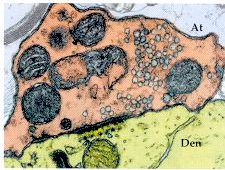
\includegraphics[width=0.1\textwidth]{images/dendrite.png}
        };

        \node[image] (n3) at ([xshift=\shifty,yshift=-1cm]mm) {
            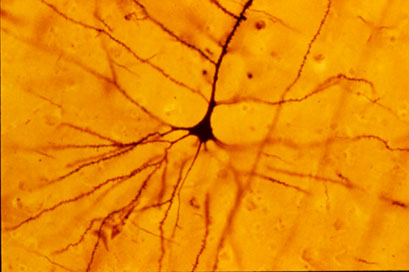
\includegraphics[width=0.1\textwidth]{images/GolgiStainedPyramidalCell.jpg}
        };

        \node[image] (n5) at ([xshift=\shifty,yshift=-1.0cm]m) {
            \includegraphics[width=0.1\textwidth]{images/brain.png}
        };

        \node[image] (n4) at ([xshift=\shifty,yshift=1cm]mm) {
            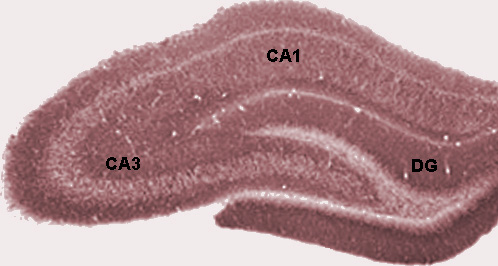
\includegraphics[width=0.1\textwidth]{images/HippocampalRegions.jpg}
        };


        \node[rectangle, minimum width=12cm, minimum height=6.0cm,
        rounded corners, opacity=0.3, fill=blue!50] (chemical) at (10.0,4.5) {};

        \node[] (caption) at ([yshift=-1cm]chemical.north) {\LARGE CHEMICAL};

        \node[rectangle, minimum width=4.5cm, minimum height=5cm
        , opacity=0.5, fill=green!50, rounded corners
            ] (electrical) at (3.8, 8.5) {};

        \node[] at (electrical.center) {\LARGE ELECTRICAL};


        % Put chemical network here
        \node[] (network) at (7.0,4.0) {
            \includegraphics[width=5cm]{images/chemical_reactions.png}
        };

        \node[] (chromosome) at (12.0,5) {
            
\includegraphics[width=5cm]{images/chromosome.png}
        };

        \node[] (text) at ([xshift=5.5cm,yshift=2cm]electrical.east) {
            \begin{minipage}{0.35\textwidth}
                \begin{itemize}[label={}]
                    \item \LARGE{$10^{11}$ cells, $10^{15}$ synapses, $\sim 10000$
                            reactions per synapse}
                    \item \LARGE{Electrical events: $\sim 1$ ms,  Chemical events: $1\;
                        \text{sec} \rightarrow 1000\; \text{sec}$}
                    \item \LARGE{Structural events: $100\; \text{sec}
                        \rightarrow \text{months}$}
                \end{itemize}
            \end{minipage}
        };
    \end{tikzpicture}  %
    \begin{tikzpicture}[scale=1 
        , every node/.style={}
        ]
        \node (moose_architecture) at (0,0) { 
            \includegraphics[width=0.5\textwidth]{./_images/moose_architecture.png}
        };
    \end{tikzpicture}


    \vspace{2cm}
    \TEXT{Specialized solvers to handle computations at different scales}
    \vspace{1cm}

    \begin{tikzpicture}
        \def\figwidth{0.12\textwidth}
        \def\captionwidth{0.25\textwidth}
        \node[] (stochastic) at ([]moose_architecture.south west) {
            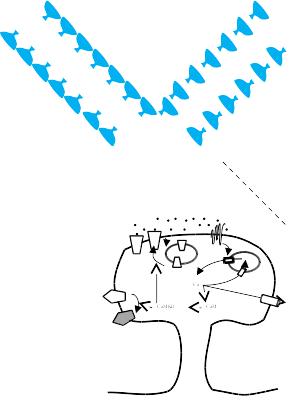
\includegraphics[height=\figwidth]{./images/stochastic_solver.png}
        }; 
        \node[text width=\captionwidth] at ([yshift=-0cm]stochastic.south)
        {\LARGE{\bf Stochastic Solver (a few molecules)}
        };
        \node[] (ksolve) at ([xshift=15cm]stochastic.east) {
            \includegraphics[height=\figwidth]{./images/ksolve_dsolve.png}
        };
        \node[text width=\captionwidth] at ([yshift=-0.0cm]ksolve.south) {
            \LARGE{\bf Reaction Diffusion Solver}};
        \node[] (hsolve) at ([xshift=15cm]ksolve.east) {
            \includegraphics[height=\figwidth]{./images/hsolve.png}
        };
        \node[text width=\captionwidth] at ([yshift=-0.0cm]hsolve.south) {
            \LARGE{\bf Electrical: Hines Solver}};
    \end{tikzpicture}

    \vspace{2cm}
    \HEADING{GUI to load/create/edit models}

    \begin{tikzpicture}[ image/.style={xslant=0.5, yslant=0.0} ]
        \node []  {
            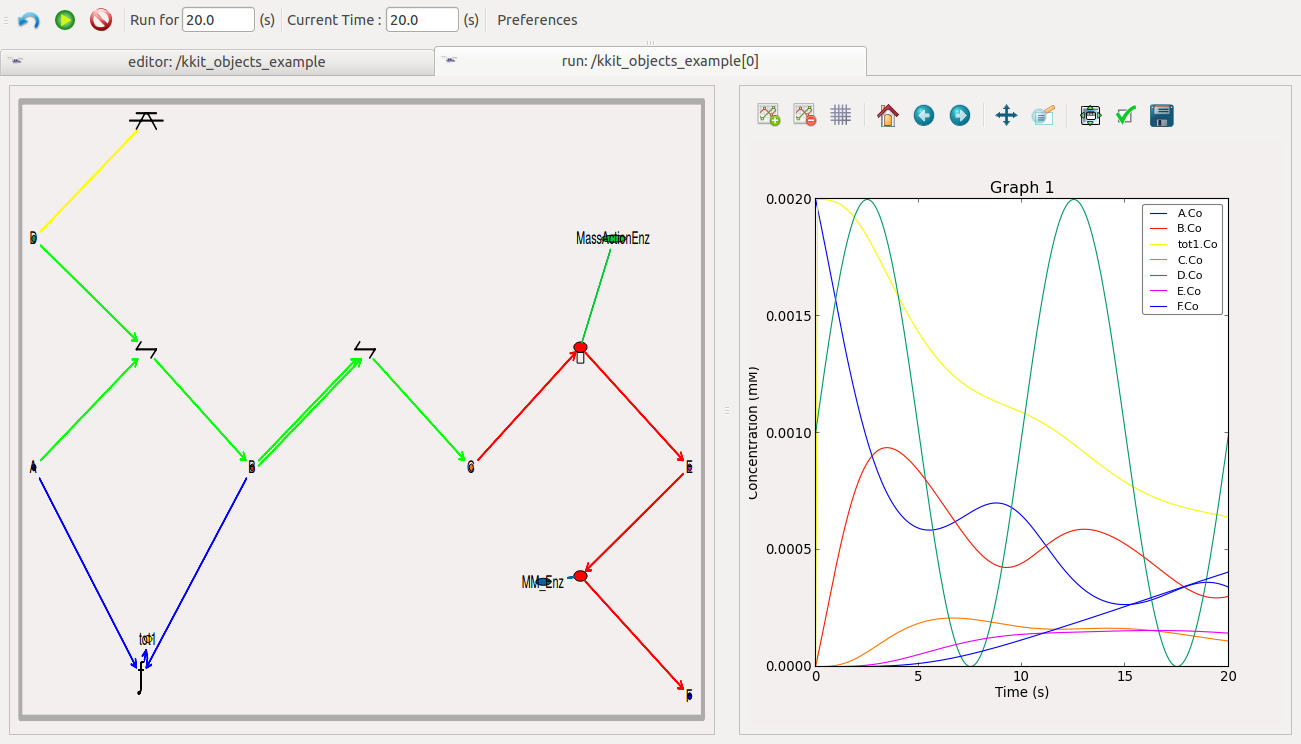
\includegraphics[width=0.5\textwidth]{./images/poster_runView.png}
        };
    \end{tikzpicture}%
    \begin{tikzpicture}
        \node [] (harsha) {
            \includegraphics[width=0.5\textwidth]{./images/moose_interface_electrical.png}
        };
    \end{tikzpicture}

    \vspace{2cm}
    \HEADING{And to play network activity}

    \begin{tikzpicture}[ image/.style={xslant=0.5, yslant=0.0} ]
        \node []  {
            \includegraphics[height=0.5\textwidth]{./images/neuron_embedded_in_network.png}
        };
    \end{tikzpicture} \hfill %
    %\begin{tikzpicture}
    %    \node [] (harsha) {
    %        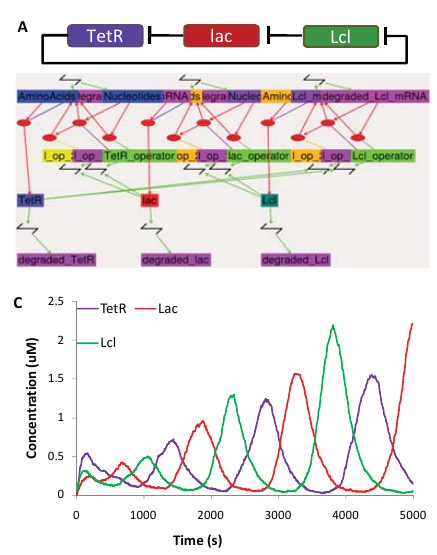
\includegraphics[width=0.8\textwidth]{./_images/reaction_diffusion_system.png}
    %    };
    %\end{tikzpicture} %
    \begin{tikzpicture}
        \node [] (networkact) {
            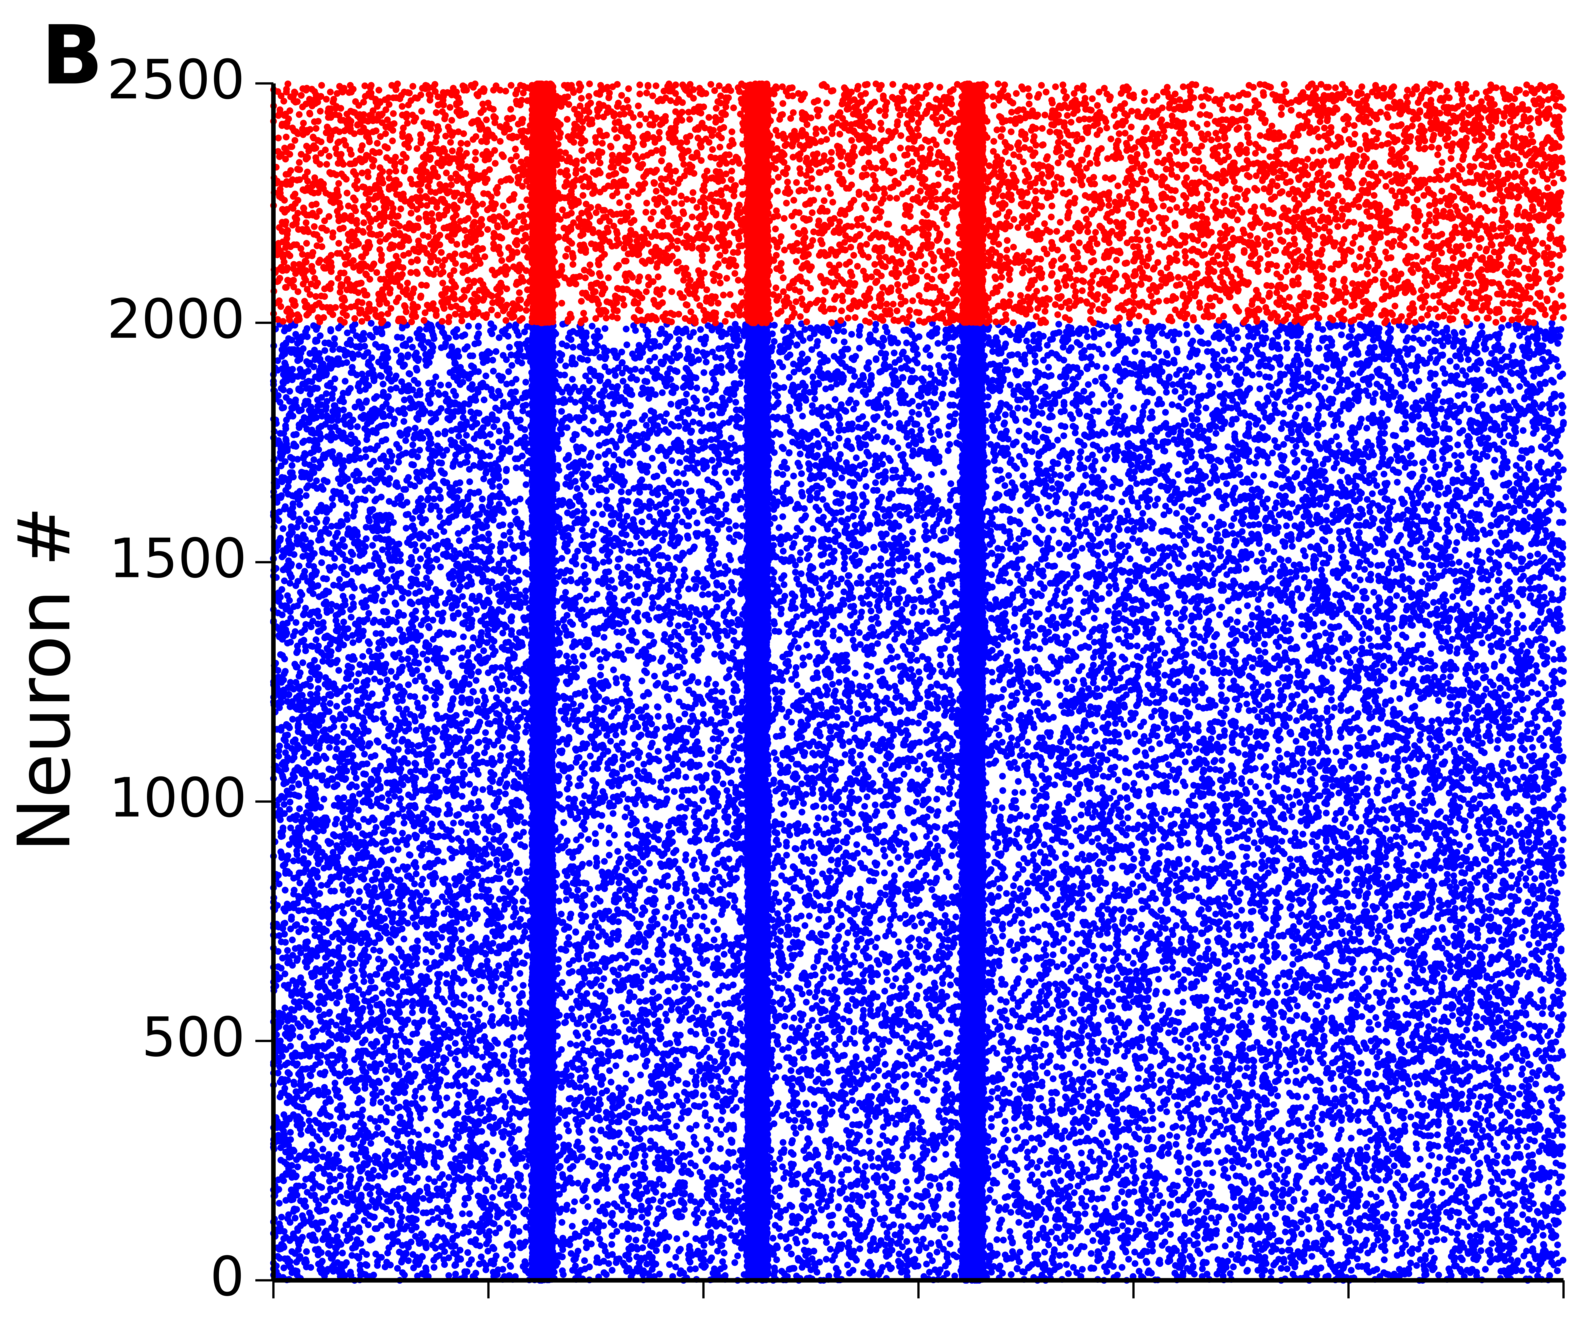
\includegraphics[width=0.6\textwidth]{./_images/panelb.png}
        };
    \end{tikzpicture}


\end{Figure}
